% vim: set spelllang=fr foldmethod=marker:
\section{Modélisation\index{modélisation}}
\label{sa:sec:modelisation}

Nous avons établi un processus de sélection aléatoire\index{selection@sélection!sélection aléatoire}, périodiquement renouvelé, des \cns assurant la détection des nœuds compromis dans le réseau.
Les simulations réalisées ont fourni des valeurs numériques permettant de valider le modèle proposé; mais elle n'ont pas la rigueur des méthodes formelles et n'offrent pas, comme ces dernières, la possibilité de vérifier de façon sure des propriétés sur l'état du système.

Dans cette section sont introduits plusieurs modèles pouvant permettre de représenter notre système, et d'en évaluer les performances selon divers critères.
Ils peuvent par ailleurs être repris pour modéliser tout système approchant.

%===============================================================================
    \subsection{Chaines de \textsc{Markov}}

        \subsubsection{Présentation et hypothèses du modèle}
En premier lieu, nous avons modélisé notre solution sous la forme d'un processus de \textsc{Markov} à temps continu (\cmtc, pour chaine de \textsc{Markov} à temps continu).
\nomenclature{CMTC}{Chaine de \textsc{Markov} à Temps Continu}
Notre modèle représente un cluster d'un \rcsf qui vérifie les hypothèses suivantes:
\begin{itemize}
    \item seul le cluster est modélisé;
    \item le cluster contient exactement un \CH; $s$ capteurs chargés d'effectuer des mesures; et $m$ nœuds jouant le rôle de \cns\,\footnote{$s$ pour \textit{sensing node}, $m$ pour \textit{monitoring node}.};
    \item il existe exactement un nœud compromis parmi les $s$ capteurs;
    \item le capteur $i$ ($1 \leq i \leq s$) génère du trafic selon un processus de \textsc{Poisson} de paramètre $\lambda_i$;
    \item le nœud compromis $c$ génère du trafic selon un processus de \textsc{Poisson} de paramètre $\lambda_c$ (tel que $\forall i\in[\![1;s]\!]\backslash\{c\},\; \lambda_c\gg\lambda_i$);
    \item chaque \cn effectue une détection du trafic environnant de façon périodique, selon une distribution exponentielle de paramètre $\mu$; si un trafic anormal est observé, le \cn transmet un rapport d'anomalie au \CH;
    \item la topologie du cluster correspond à un graphe connexe: chaque nœud peut atteindre directement chacun des autres nœuds du cluster.
\end{itemize}

        \subsubsection{Modélisation\index{modélisation}}
Sous les hypothèses précédentes, notre modèle peut être représenté par une \cmtc multidimensionnelle de taille $m$.
Il est alors exprimé sous la forme d'un $m$-uplet $x\!=\!(x_1,x_2,\dots,x_m)$ de macro-états $x_k\!=\!(x_{k_1},x_{k_2},\dots,x_{k_s},x_{k_d})$.
Chaque macro-état $x_k$ représente le nombre de paquets détectés par le \cn $k$ ($1\leq k\leq m$).
Plus exactement, chaque $x_{k_i}$ ($1\leq i\leq s$) est un compteur, initialisé à $0$, qui est incrémenté à chaque fois que le \cn $k$ détecte un paquet en provenance du capteur $i$.
$x_{k_d}$ est une variable de type booléen, initialisée à $0$, et passée à $1$ lorsque le \cn $k$ détecte un trafic anormalement élevé.
La fonction de seuil $f:s^s\rightarrow\{0;1\}$ est utilisée par les \cns pour déterminer la nature normale ou non du trafic (elle indique si un paquet a dépassé ou non le seuil des communications dites «normales»).
Elle prend pour argument les valeurs des $s$ compteurs $x_{k_1},x_{k_2},\dots,x_{k_s}$ d'un macro-état $x_k$ associé à un \cn $k$, et la valeur retournée est stockée dans $x_{k_d}$.

\newlength\fboxlinelen
\setlength\fboxlinelen\linewidth
\addtolength\fboxlinelen{-2\fboxsep}
\addtolength\fboxlinelen{-2\fboxrule}
\begin{figure}[ht]
    \fbox{%
        \begin{minipage}{\fboxlinelen}
            \newlength\backupads
            \setlength\backupads\abovedisplayskip
            \setlength\abovedisplayskip{0pt}
            \begin{eqnarray*}
                x_k    & \rightarrow & \mbox{Transmission d'un capteur normal} \\
                    & \rightarrow & (x_{k_1},\dots,x_{k_i}+1,\dots,x_{k_c},  \dots,x_{k_s},0) \\
                    &             & \qquad\mbox{avec la fréquence }\lambda_{i}\!\neq\!\lambda_{c} \\ \\
                    & \rightarrow & \mbox{Transmission du nœud compromis} \\
                    & \rightarrow & (x_{k_1},\dots,x_{k_i},  \dots,x_{k_c}+1,\dots,x_{k_s},0) \\
                    &             & \qquad\mbox{avec la fréquence }\lambda_{c}\\ \\
                    & \rightarrow & \mbox{Vérification; détection d'un trafic anormal}\\
                    & \rightarrow & (0,\dots,0,\dots,0,\dots,0,1) \\
                    &             & \qquad\mbox{avec la fréquence }\mu \cdot 1_{f(x_k)\geq \mathit{seuil}} \\ \\
                    & \rightarrow & \mbox{Vérification; aucun trafic anormal détecté} \\
                    & \rightarrow & (0,\dots,0,\dots,0,\dots,0,0)  \\
                    &             & \qquad\mbox{avec la fréquence }\mu \cdot 1_{f(x_k)<\mathit{seuil}}
            \end{eqnarray*}
            \setlength\abovedisplayskip\backupads
        \end{minipage}%
    }
    \caption{Exemple d'équation de transition du processus de \textsc{Markov} à temps continu modélisant le cluster}\label{sa:fig:eqtrans}
\end{figure}

Nous donnons un exemple d'équation de transition pour un macro-état générique $x_k$, $1\leq k\leq m$.
Le macro-état $x$, représentant l'intégralité du système, est directement obtenu en agrégeant les différents $x_k$.
Le compteur $x_{k_c}$ représente dans la suite le nombre de messages émis par le nœud compromis et captés par le \cn $k$.
L'équation est donnée en \figref{sa:fig:eqtrans}.

Formulé autrement: le \cn $k$, dans l'état $x_k$, reçoit périodiquement les messages de chaque capteur $i$ (pour tout $i$ tel que $1\leq i\leq s, i\!\neq\!k$): ce sont des transmissions dites «normales», qui surviennent avec une fréquence moyenne $\lambda_i$.
Chaque message reçu laisse le \cn $k$ dans un état presque identique, à la seule différence que le compteur $x_{k_i}$ est incrémenté de $1$.
La même chose se produit avec une fréquence $\lambda_c$ pour les messages envoyés par le nœud compromis, qui provoque à chaque fois l'incrémentation du compteur $x_{k_c}$.
Enfin, la vérification du trafic enregistré par le \cn $k$ survient avec une fréquence $\mu$.
La fonction $f$ est appliquée sur l'ensemble des $x_{k_i}$, $i$ allant de $1$ à $s$.
Si l'un des capteurs a envoyé un nombre de paquets supérieur à la valeur de seuil (\cad si l'on a $f(x_k)\geq \mathit{seuil}$), le drapeau $x_{k_d}$ est levé.
Un message d'alerte est alors envoyé du \cn $k$ au \ch.
Si, en revanche, aucune anomalie n'est à rapporter, le drapeau $x_{k_i}$ est laissé à $0$, et rien n'est envoyé.
Dans les deux cas, tous les compteurs $x_{k_i}$ sont réinitialisés à $0$, afin que la prochaine vérification soit effectuée sur des données «fraiches» (et pour ne pas déclencher par erreur une fausse détection par cumul des nombres de paquets envoyés d'une période sur l'autre).

La probabilité de détection du nœud compromis par le \cn $k$, notée $\Delta_k$, est la suivante:
\[\Delta_k=\sum_{x_{k_1},\dots,x_{k_s}}^\infty\pi(x_{k_1},\dots,x_{k_s},x_{k_d}=1)\]
où la valeur \quad$\pi(x_{k_1},x_{k_2},\dots,x_{k_{s}},x_{k_d})$\quad représente la distribution stationnaire du macro-état $x_k\!=\!(x_{k_1},x_{k_2},\dots,x_{k_{s}},x_{k_d})$.

        \subsubsection{Limites du modèle}
Représenté sous la forme d'un processus de \textsc{Markov} à temps continu, le modèle suppose que la période séparant deux vérifications consécutives du trafic par un \cn est une variable aléatoire qui suit une distribution exponentielle.
Il s'agit là d'une approximation grossière; en réalité, la vérification intervient à intervalles réguliers (de longueur fixe), voire même en continu.
Il est donc nécessaire de choisir d'autres systèmes que les processus de \textsc{Markov} pour modéliser notre solution avec plus de précision.
Nous allons ainsi nous orienter vers des processus non-markoviens, qui ne présentent pas cette contrainte.

%===============================================================================
    \subsection{Réseaux de \textsc{Petri}}

Une autre représentation possible du système passe ainsi par l'utilisation de processus stochastiques à évènements discrets (PSED, en anglais \textit{Discrete-Event Stochastic Processes}, ou encore \textit{Generalized Semi-\textsc{Markov} Processes} pour «processus semi-markoviens généralisés»).
Leur avantage principal sur les processus de \textsc{Markov} est leur capacité à représenter des évènements dont la distribution n'est pas nécessairement exponentielle.
Plus particulièrement, nous allons utiliser des réseaux de \textsc{Petri} stochastiques généralisés étendus.
\nomenclature{PSED}{Processus Stochastiques à Évènements Discrets}

        \subsubsection{Réseaux de \textsc{Petri} stochastiques généralisés étendus}
\label{sa:subsubsec:presRPSGe}
Les réseaux de \textsc{Petri} stochastiques généralisés (\rpsg) forment une classe de réseaux de \textsc{Petri} destinée à modéliser des processus stochastiques.
Leur version étendue (\rpsge) permet de représenter des transitions dont les délais sont distribués de façon quelconque~\cite{ABCDF95}.
Il s'agit d'un langage de haut niveau permettant de représenter des processus stochastiques à évènements discrets, qui au contraire des processus markoviens «classiques» ne sont pas limités à la représentation d'évènements à distribution exponentielle.
\rpsge reprend, à quelques différences près, les définitions, la syntaxe et la représentation graphique des réseaux de \textsc{Petri} classiques, enrichis par des propriétés supplémentaires portant sur les transitions.
Ces dernières sont dites soit \textit{immédiates}, soit \textit{minutées}.
Elles sont de plus caractérisées par les éléments suivants:
\begin{enumerate}
    \item une distribution qui détermine de façon aléatoire le délai écoulé avant que la transition ne soit franchie;
    \item une priorité qui établit de façon déterministe la transition à franchir en premier, en cas d'égalité;
    \item un poids qui est utilisé pour tirer de façon aléatoire la transition à franchir en premier, en cas de conflits sur le délai écoulé et sur les priorités.
\end{enumerate}
\nomenclature{RPSG}{Réseaux de \textsc{Petri} Stochastiques Généralisés}
\nomenclature{RPSGe}{Réseaux de \textsc{Petri} Stochastiques Généralisés étendus}

Nous utilisons deux types de transitions minutées:
\begin{itemize}
    \item les distributions minutées exponentiellement distribuées (marquées dans les figures qui suivent par des rectangles vides, voir par exemple la transition \textsf{T1} sur l'exemple de gauche de la \figref{sa:fig:gspnex1});
    \item les distributions minutées distribuées de façon déterministe (marquées dans les figures qui suivent par des rectangles bleus, voir par exemple la transition \textsf{T1} sur l'exemple de droite de la \figref{sa:fig:gspnex1}).
\end{itemize}
Les transitions immédiates sont marquées par des rectangles pleins et noirs (voir par exemple la transition \textsf{T2} dans les exemples de la \figref{sa:fig:gspnex1}).
Nous avons aussi recours à des arcs inhibiteurs.
Il s'agit d'arêtes dont la flèche sur les représentations graphiques est remplacée par un cercle (par exemple, l'arc reliant la place \textsf{P1} à la transition \textsf{T2} dans l'exemple de droite de la \figref{sa:fig:gspnex1}), et accompagnées d'un chiffre.
Les règles de franchissement des transitions sont légèrement différentes avec ces arcs, puisque ces franchissements ne peuvent être effectués que si le nombre de jetons en amont de la transition est strictement inférieur au nombre indiqué sur l'arc.
Par exemple, sur la partie droite de la \figref{sa:fig:gspnex1}, la transition \textsf{T2} peut être franchie, car \textsf{P1} ne contient que deux jetons (on a bien $2<3$).
\begin{figure}[ht]
    \centering
    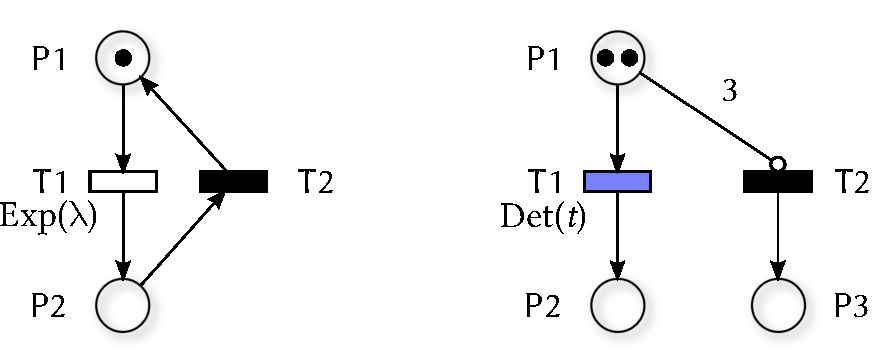
\includegraphics[width=.8\linewidth]{\chapterfig/RPSGe_example.pdf}
    \caption{Exemples simples de \rpsge: transitions immédiates, transitions minutées et arcs inhibiteurs}\label{sa:fig:gspnex1}
\end{figure}

        \subsubsection{Modélisation\index{modélisation} des nœuds}
Nous allons procéder par étapes en modélisant:
\begin{enumerate}
    \item les nœuds capteurs «simples»;
    \item les \cns désignés de manière statique;
    \item les \cns désignés de façon dynamique (dont la \idx{modélisation} diffère légèrement).
\end{enumerate}

            \paragraph{Modélisation\index{modélisation} des capteurs simples}
Le comportement des capteurs basiques (qui poursuivent simplement leur mission de récolte de données) est simple: chaque capteur $i$ envoie des paquets selon un processus de \textsc{Poisson} de paramètre $\lambda_i$.
Ce comportement est modélisé par le \rpsg présenté en \figref{sa:fig:snodegspn}.
Le nœud y est symbolisé par les pointillés bleus.
Dans ce nœud $i$ se trouve une unique transition \textsf{TX}, sans place en entrée, autrement dit: toujours active.
Elle est minutée, avec une distribution exponentielle de paramètre $\lambda_i$: chaque évènement correspond à l'envoi de jetons sur tous ses arcs sortants.
Ces arcs sont rattachés à la place \textsf{InBuff$_{j}$}\,\footnote{Pour \textit{in buffer}.} de chacun des nœuds voisins du nœud $i$ (on trouve donc autant d'arcs sortants que de nœuds voisins).
L'intégralité de la fonction de mesure et d'envoi des données utiles du \rc peut être modélisée par plusieurs éléments représentés par ce «modèle de nœud».
Un nœud compromis $c$ sera également représenté selon le même modèle, avec un paramètre $\lambda_c$ plus élevé que les autres $\lambda_i$.
\begin{figure}[!ht]
    \centering
    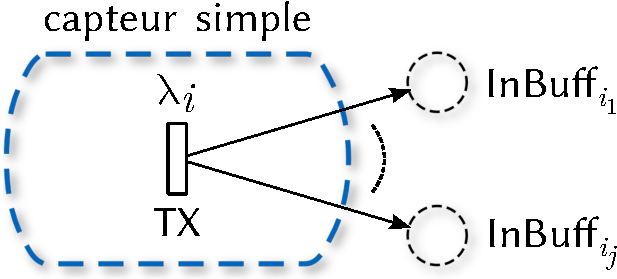
\includegraphics[width=.5\linewidth]{\chapterfig/RPSGe_sensing.pdf}
    \caption{Modèle \rpsg d'un nœud capteur simple}\label{sa:fig:snodegspn}
\end{figure}

            \paragraph{Modélisation\index{modélisation} du \ch}
Nous travaillons de l'intérieur du cluster, et le \ch est vu comme un simple puits qui reçoit les paquets émis par les autres nœuds.
Son activité de retransmission à destination de la \sdb n'est donc pas représentée.
Illustré en \figref{sa:fig:chgspn}, le \CH ne contient donc qu'une place \textsf{InBuff$_\textsf{CH}$} qui représente le tampon contenant les messages reçus, et reliée aux transitions \textsf{TX$_i$} de tous les autres nœuds.
\begin{figure}[ht]
    \centering
    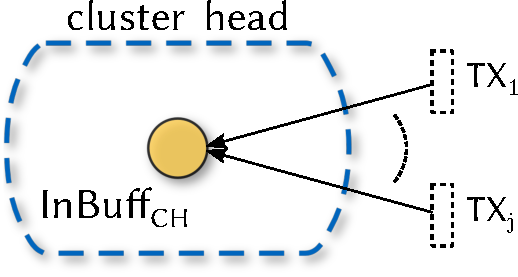
\includegraphics[width=.45\linewidth]{\chapterfig/RPSGe_CH.pdf}
    \caption{Modèle \rpsg du \ch}\label{sa:fig:chgspn}
\end{figure}
En réalité, il devrait y avoir une place \textsf{InBuff$_i$} distincte pour les jetons provenant de chaque nœud voisin $i$ du \ch. Pour simplifier la représentation, tous les jetons arrivant au modèle du nœud sont rassemblés dans une place unique.

            \paragraph{Modélisation\index{modélisation} des \cns désignés de façon statique}
Un \cn élu de façon statique joue uniquement son rôle de \cn: il écoute le trafic, mais n'effectue pas de mesures sur son environnement.
Le modèle \rpsge associé à ce type de nœud est présenté en \figref{sa:fig:cnodegspn1}.
La place \textsf{InBuff} représente le tampon contenant les messages reçus par le nœud.
Un jeton arrivant dans cette place (depuis un nœud «normal») représente un message capté par le \cn.
La vérification du respect de la valeur seuil $K$ pour le trafic est réalisée à intervalles de temps constants.
Les transitions \textsf{vérif\_OUI} et \textsf{vérif\_NON} sont «activées» au bout de chaque période, et servent à assurer la vérification.
S'il y a au moins $K$ jetons dans la place, la transition \textsf{vérif\_OUI} est franchie.
Un jeton est alors placé dans la place \textsf{det}, et fait en quelque sorte office de drapeau levé pour indiquer la détection d'un trafic anormal.
L'arrivée d'un jeton dans la place \textsf{det} déclenche l'envoi d'un message d'alerte au \ch.
Si, en revanche, il y a moins de $K$ jetons dans la place \textsf{InBuff}, aucun jeton n'est produit dans la place \textsf{det}.
Dans un cas comme dans l'autre, la place \textsf{vider~tampon} reçoit un jeton (soit par \textsf{vérif\_OUI}, soit par \textsf{vérif\_NON}).
Un jeton dans cette place permet de vider le tampon \textsf{InBuff}: la transition \textsf{e-déb} consomme le jeton de la place \textsf{vider~tampon}, et un jeton de \textsf{InBuff}.
Un nouveau jeton est créé dans \textsf{vider~tampon}.
Le processus est répété jusqu'à ce que la place \textsf{InBuff} soit vide; dans ce cas, la transition \textsf{e-fin} est franchie et ne produit rien, mais met fin à la consommation des jetons.
Les étapes permettant de vider le tampon ne consomment pas de temps, et permettent de repartir avec un compteur neutre pour la période qui mènera à la vérifiation suivante.
\begin{figure}[ht]
    \centering
    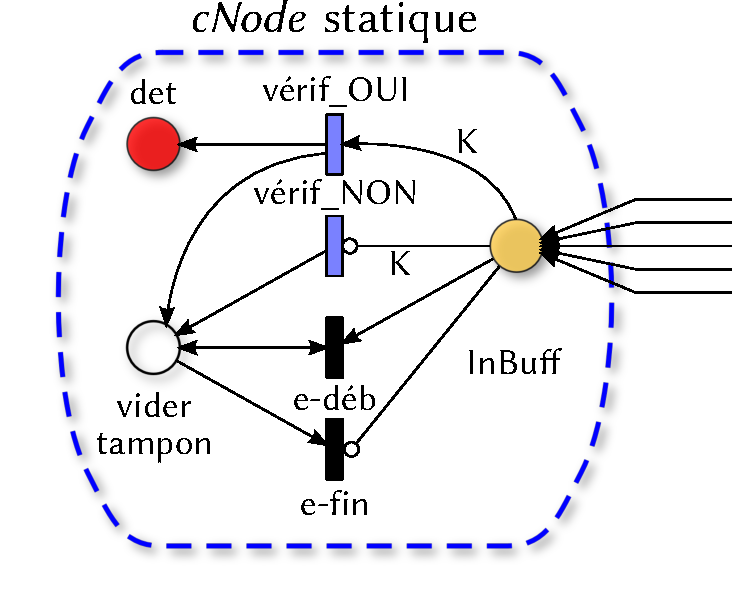
\includegraphics[width=.54\linewidth]{\chapterfig/RPSGe_cNode_static.pdf}
    \caption{Modèle \rpsge d'un \cn élu de manière \emph{statique}}\label{sa:fig:cnodegspn1}
\end{figure}

            \paragraph{Modélisation\index{modélisation} des \cns désignés de façon dynamique}
Le modèle \rpsge représentant le \cn élu de façon dynamique ressemble à son homologue élu de façon statique.
Cependant, en raison de l'\elecdyn, tous les nœuds vont assumer périodiquement le rôle de \cn et le rôle de capteur simple.
Il est donc nécessaire d'ajouter, aux places et transitions des précédents \cns, une place \textsf{cNode} ainsi qu'une transition toujours autorisée, associée à une distribution exponentielle.
La première permet d'indiquer à chaque instant si le nœud joue le rôle de \cn (si la place contient un jeton) ou bien de capteur simple (cas contraire).
La seconde permet de produire des jetons selon un processus de \textsc{Poisson} lorsque le nœud fait office de capteur simple (dans ce cas la place \textsf{cNode} est vide et l'arc inhibiteur autorise le franchissement de la transition \textsf{TX}; le nœud se comporte exactement comme avec le modèle de la \figref{sa:fig:snodegspn}).
Le modèle est représenté sur la \figref{sa:fig:cnodegspn2}.
\begin{figure}[!ht]
    \centering
    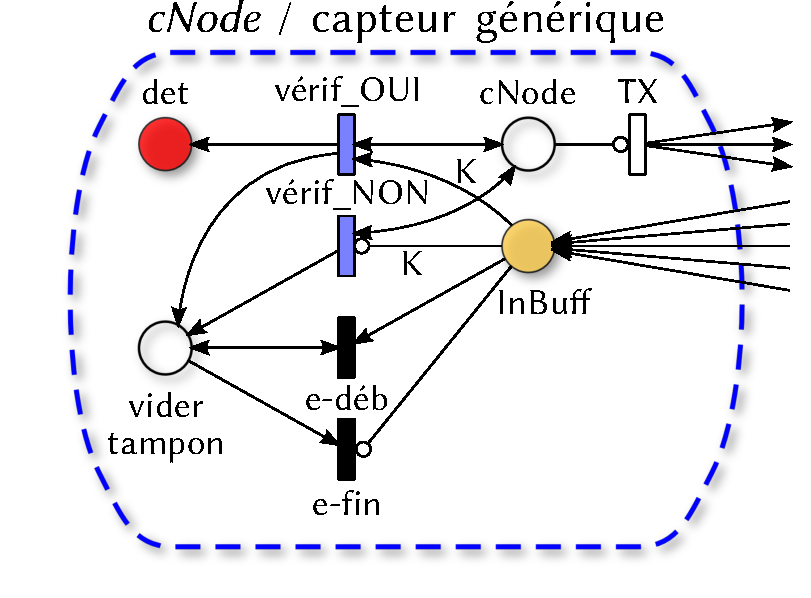
\includegraphics[width=.6\linewidth]{\chapterfig/RPSGe_cNode_generic.pdf}
    \caption{Modèle \rpsge d'un \cn élu de manière \emph{dynamique}}\label{sa:fig:cnodegspn2}
\end{figure}

        \subsubsection{Modélisation\index{modélisation} du cluster}

            \paragraph{\cns désignés de façon statique}
Maintenant que la représentation des nœuds individuels a été donnée, nous sommes en mesure de modéliser notre cluster.
Pour simplifier la représentation graphique, nous choisissons de représenter un cluster comportant un total de neuf nœuds placés sur une grille de dimensions $3\times3$.
Parmi ces nœuds, deux exactement jouent le rôle de \cn (les nœuds \textsf{3} et \textsf{4} dans notre cas), et un exactement (le nœud \textsf{1}) est un capteur compromis (distinct des \cns).
Le nœud \textsf{5} quant à lui tient le rôle du \ch.
La représentation du cluster est donnée en \figref{sa:fig:petricluster}.
Également dans l'optique de simplifier la représentation graphique, les transitions \textsf{e-déb} et \textsf{e-fin}, ainsi que la place \textsf{vider~tampon}, ont été remplacées par une boite blanche associée à la fonction de vidage de la place \textsf{InBuff} des nœuds.
Cette représentation peut être facilement étendue pour modéliser le réseau tout entier.
On observera, par rapport au modèle précédent basé sur les chaines de \textsc{Markov}, que le graphe du cluster n'est plus connexe: les nœuds ne peuvent atteindre que leurs voisins directs (sur le côté ou en diagonale sur la représentation).
Là encore, il s'agit d'un choix permettant de simplifier le graphique, et la connexité du réseau peut être complétée par le simple ajout des arêtes manquantes.
\begin{figure}[!ht]
    \centering
    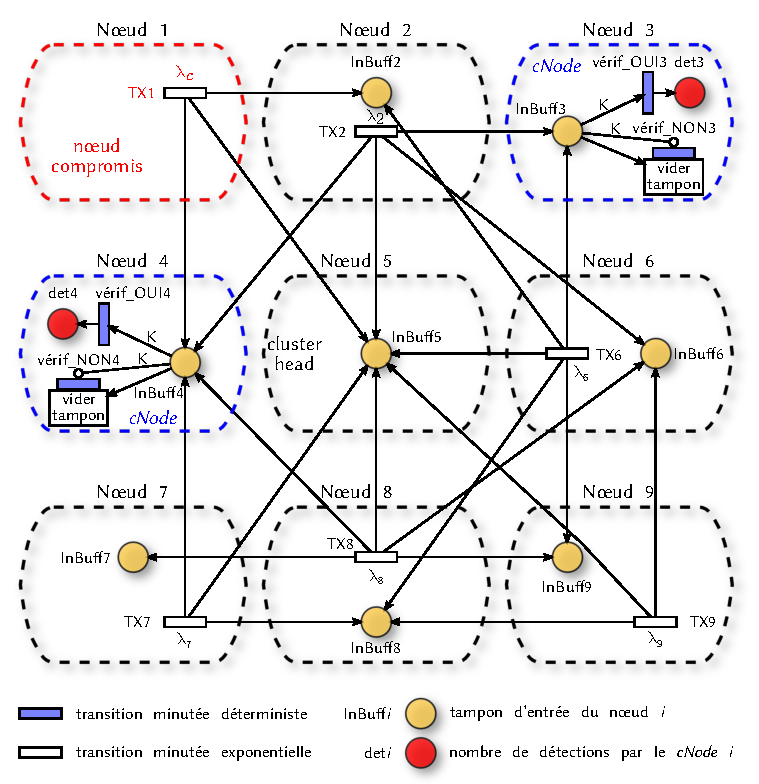
\includegraphics[width=\linewidth]{\chapterfig/RPSGe_network3x3_static.pdf}
    \caption{Modèle \rpsge d'un cluster (topologie: grille $3\times3$) comprenant un nœud compromis et deux \cns statiques}\label{sa:fig:petricluster}
\end{figure}

            \paragraph{\cns désignés de façon dynamique}
L'\elecdyn des \cns vient compliquer légèrement la \idx{modélisation} de notre cluster.
Bien évidemment, tous les nœuds seront représentés selon le modèle ambivalent illustré par la \figref{sa:fig:cnodegspn2}.
Mais il est aussi nécessaire de rajouter un module qui permettra l'\election des \cns pour chaque période.
Pour une meilleure clarté, le cluster sera représenté en deux temps.

Tout d'abord, la \figref{sa:fig:petridyn} représente le cluster comme nous l'avons vu jusqu'ici, sous formes de nœud distincts et de transitions représentant le trafic émis.
Les sept nœuds non compromis peuvent endosser alternativement les rôles de capteur simple et de \cn (leur représentation a été simplifiée par rapport à la \figref{sa:fig:cnodegspn2}).
Le \ch n'est toujours considéré que comme un simple puits, uniquement équipé d'un tampon mémoire d'entrée pour recevoir les données.
\begin{figure}[!b]
    \centering
    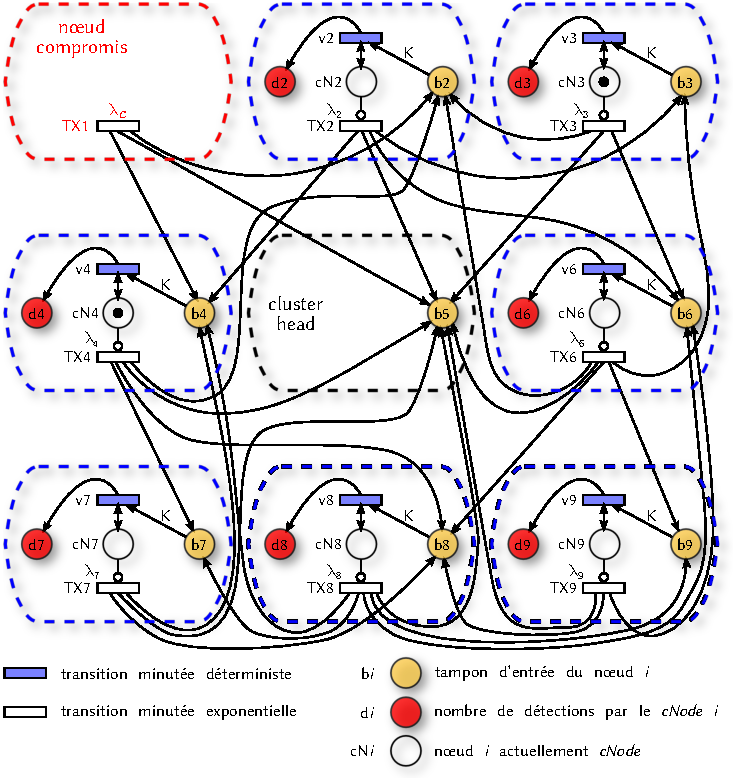
\includegraphics[width=\linewidth]{\chapterfig/RPSGe_network3x3_dynamic.pdf}
    \caption{Modèle \rpsge pour le trafic d'un cluster (topologie: grille $3\times3$) comprenant un nœud compromis et deux \cns sélectionnés de façon dynamique}\label{sa:fig:petridyn}
\end{figure}

Un second réseau de \textsc{Petri} est utilisé pour modéliser le processus de sélection\index{selection@sélection} lui-même.
En considérant $n$ comme le nombre de résultats possibles à l'\election, le module représentant l'\elecdyn des \cns comprend:
\begin{itemize}
    \item une unique place centrale;
    \item $n$ transitions minutées, suivant une distribution déterministe, et mutuellement exclusives, menant à cette place (en bleu sur la \figref{sa:fig:petrielec});
    \item $n$ transitions immédiates et mutuellement exclusives, franchissables depuis la place centrale (en noir sur la \figref{sa:fig:petrielec}).
\end{itemize}
Dans notre cas, pour choisir deux \cns au sein du cluster, et en supposant que le nœud compromis ne peut être désigné, nous avons $n=\binom{7}{2}=21$~issues possibles pour l'\election.
À la fin d'une période d'activité des \cns, une nouvelle \election est déclenchée.
La transition minutée correspondant aux \cns sélectionnés pour la période qui s'achève est déclenchée; les jetons présents dans les places \textsf{cNode} de ces \cns sont consommés, et produisent ainsi un jeton dans l'unique place centrale du module.
Chaque transition immédiate tente alors de produire un jeton.
Comme elles sont mutuellement exclusives, mais ont la même priorité et le même poids (voir \sssref{sa:subsubsec:presRPSGe}), un tirage aléatoire a lieu pour déterminer l'unique transition qui est franchie et qui produit ses jetons.
Ceux-ci sont envoyés dans les places \textsf{cNode} des nœuds sélectionnés pour la période qui débute, activant ainsi leurs fonctionnalités de \cns.
\begin{figure}[!ht]
    \centering
    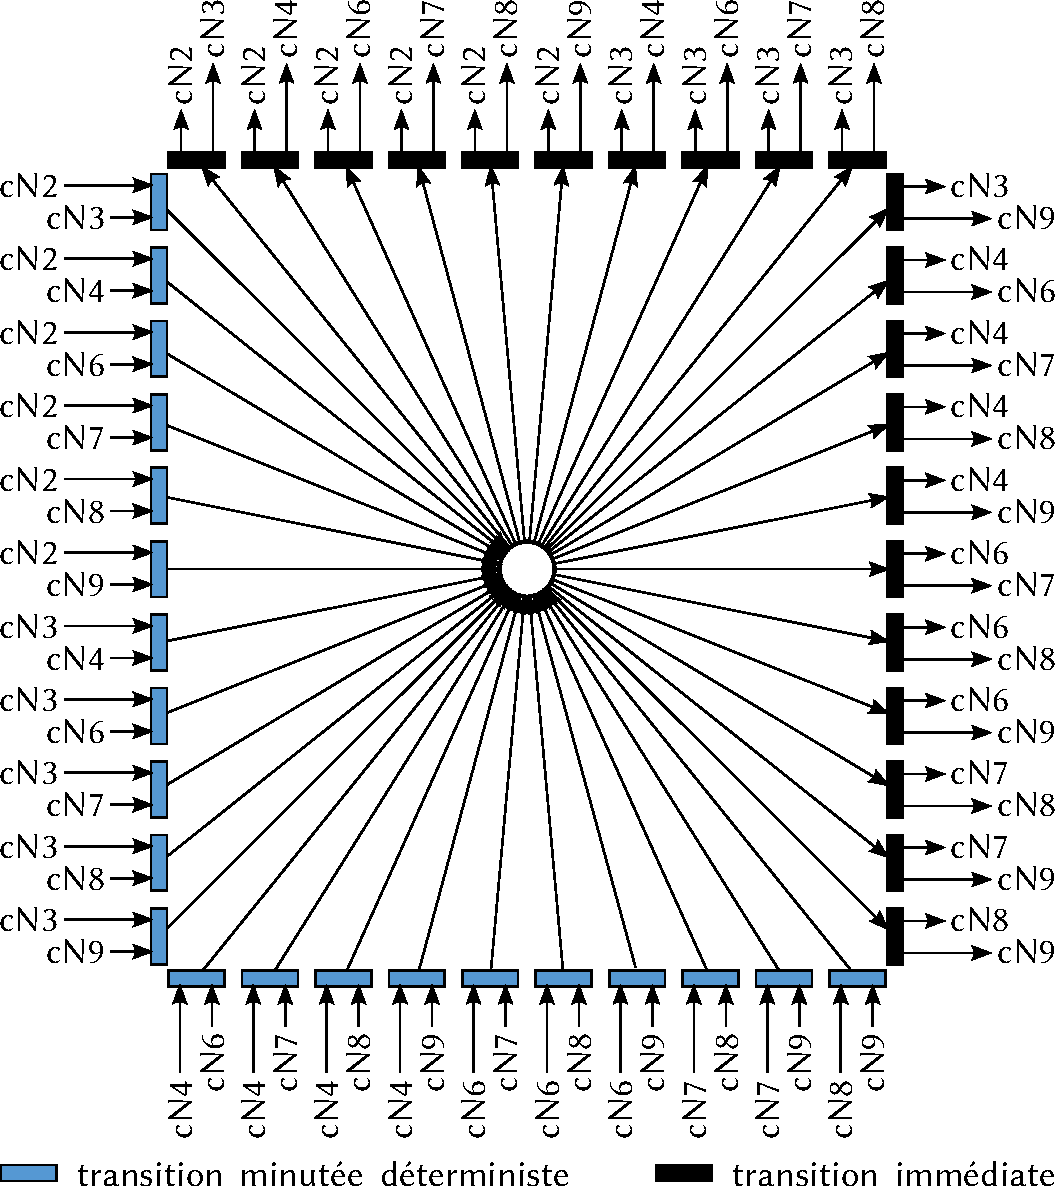
\includegraphics[width=.9\linewidth]{\chapterfig/RPSGe_network3x3_selection.pdf}
    \caption{Modèle \rpsge pour l'\elecdyn de deux \cns parmi les nœuds du cluster}\label{sa:fig:petrielec}
\end{figure}
%===============================================================================
    \subsection{Logique stochastique avec automates hybrides}

        \subsubsection{Présentation de la logique stochastique avec automates hybrides}
La logique stochastique avec automates hybrides (\lsah; \textit{Hybrid Automata Stochastic Logic} en anglais) est un langage récent, qui introduit une architecture regroupant des études de \modelchecking et d'évaluation des performances ainsi que de fiabilité sur des processus stochastiques à évènements discrets (PSED) exprimés sous forme de réseaux de \textsc{Petri} stochastiques généralisés (\rpsg)~\cite{BDDHP11hasl}.
Plus concrètement, à partir d'un modèle \rpsg, les mesures de performances sont exprimées à l'aide de formules \lsah avant que leur soient appliquées des fonctions de \modelchecking statique permettant de vérifier automatiquement ces formules.
%en place de vérifications, en termes d'études statistiques, de modèles stochastiques~\cite{BDDHP11hasl}.
\nomenclature{LSAH}{Logique Stochastique avec Automates Hybrides}

Pour bien comprendre le fonctionnement de \lsah, voici quelques rappels sur le \modelchecking.
Il s'agit d'une procédure de vérification formelle utilisant:
\begin{itemize}
    \item un modèle $M$ à états discrets;
    \item une propriété formelle exprimée par une formule de logique temporelle $\phi$.
\end{itemize}
Un algorithme est alors utilisé pour déterminer automatiquement si $\phi$ vérifie $M$ (ce que l'on note $M\models\phi$).
Dans le cas d'un modèle stochastique, des probabilités sont associées aux formules.
Vérifier que $M\models\phi$ revient alors à déterminer la probabilité de la formule $\phi$ dans le contexte du modèle $M$\kern-1pt.
\lsah étend ce concept dans le sens où l'évaluation d'une formule peut donner n'importe quel nombre réel, et représenter ainsi une probabilité aussi bien que toute autre mesure de performance.
À cette fin, \lsah fait appel à des automates linéaires hybrides (\alh).
\nomenclature{ALH}{Automate Linéaire Hybride}
Un \alh résulte, de manière résumée, de la généralisation des automates temporels dont les variables «horloges» sont remplacées par des variables de données réellement évaluées.
Basée sur ce modèle une formule \lsah comprend ainsi deux sous-éléments:
\begin{itemize}
    \item un \alh permettant la sélection des exécutions temporelles à retenir à partir du modèle \rpsg considéré, cette sélection étant le fruit de la synchronisation entre une exécution générée par le modèle \rpsg et l'\alh;
    \item une expression $Z$, représentant la mesure à évaluer, construite à l'aide des variables de l'\alh selon la syntaxe suivante:
    \[
        \begin{split}
            Z ::=  & \ E(Y)\ | \ Z+Z\           | \ Z \times Z\\
            Y ::=  & \ c\    | \ Y+Y\           | \ Y \times Y\    | \ Y/Y\            | \ \mbox{dern}(y)\ | \ \mbox{min}(y)\\
                   & \ \     | \ \mbox{max}(y)\ | \ \mbox{int}(y)\ | \ \mbox{moy}(y)\\
            y ::=  & \ c\    | \ x\             | \ y+y\           | \ y \times y\     | \ y/y
        \end{split}
    \]
    Cette expression peut être interprétée comme suit:
    \begin{itemize}
        \item $x$ est une variable de données de l'automate:
        \item $y$ est une expression arithmétique à partir de ces variables de données;
        \item $Y$ est une variable de chemin aléatoire, \cad une variable évaluée à l'aide d'un chemin de synchronisation, lui-même créé par la synchronisation entre une trajectoire du modèle \rpsg et l'\alh;
        \item $\mbox{dern}(y)$ est la dernière des valeurs endossées par l'expression $y$ le long d'un chemin synchronisé; $\mbox{min}(y)$ et $\mbox{max}(y)$ sont les valeurs optimales obtenues le long de ce chemin; $\mbox{int}(y)$ est l'intégrale d'$y$, et $\mbox{moy}(y)$ la moyenne des valeurs obtenues le long du chemin.
    \end{itemize}
\end{itemize}

Au final, \lsah fonctionne de la façon suivante:
\begin{enumerate}
    \item le système est exprimé sous la forme d'un modèle \rpsg et d'une formule \lsah;
    \item \lsah génère de façon itérative les trajectoires à partir de l'espace d'états du modèle \rpsg et les synchronise avec l'\alh;
    \item les trajectoires acceptées par l'\alh sont évaluées pour obtenir l'estimation de la mesure étudiée. Les trajectoires refusées sont abandonnées.
\end{enumerate}

        \subsubsection{Automate linéaire hybride et formule \lsah associés au modèle utilisé}
Nous présentons ici quelques exemples de formules \lsah, constitués des expressions \lsah et d'un automate linéaire hybride (\alh) associé au modèle \rpsge présenté plus haut (en \figref{sa:fig:petridyn}).
Ces exemples présentent une manière de mesurer des données sur un nœud du \rc à partir de la version modélisée sous forme de réseaux de \textsc{Petri}, à fin d'étude, ou bien de comparaison de notre solution avec d'autres systèmes de détection\index{système de détection d'intrusion} des attaques par \dds.
Ces exemples peuvent en outre être modélisés facilement avec l'outil de \modelchecking \textsf{COSMOS}~\cite{BDDHP11cosmos}.

On considère un nœud quelconque $i$ ($1\leq i\leq$~nombre de capteurs).
L'automate linéaire hybride que nous utilisons fait appel aux variables suivantes:
\begin{itemize}
    \item $x_t$: temps global;
    \item $x_{d_i}$: nombre d'attaques détectées par le \cn $i$;
    \item $x_{\mathsf{TX}_i}$: nombre de paquets envoyés par le nœud $i$;
    \item $x_{\mathit{bf}_i}$: nombre de paquets reçus et placés dans le tampon en entrée du nœud $i$.
\end{itemize}
L'automate linéaire hybride est présenté en \figref{sa:fig:lha}.
\begin{figure}[!b]
    \fbox{%
        \begin{minipage}{\fboxlinelen}
            \centering
            \begin{tikzpicture}[auto, thick, >=stealth]
                \node[state, minimum width=7.5em, inner sep=-5em] (a) at (0,0) {%
                    \hspace{.5em}
                    \mbox{%
                        \begin{tabular}{l @{}c @{ }l}
                            $\dot{x}_t$               & : & $1$\\
                            $\dot{x}_{d_i}$           & : & $0$\\
                            $\dot{x}_{\textit{bf}_i}$ & : & $M(\textit{bf}_i)$\\
                            $\dot{x}_{\textsf{TX}_i}$ & : & $0$\\
                        \end{tabular}%
                    }
                };

                \node[state, minimum width=7.5em, accepting] (b) at (6,0) {};

                \draw[->] (a) edge[loop above, looseness=6] %
                node[] {$\textit{vrai}, \{\textsf{vérif\_OUI}_i\}, (x_{d_i}:=x_{d_i}+1)$} (a);
                \draw[->] (a) edge[loop below, looseness=6] %
                node[] {$\textit{vrai}, \{\textsf{TX}_i\}, (x_{\textsf{TX}_i}:=x_{\textsf{TX}_i}+1$)} (a);
                \draw[->] (a) edge[above] %
                node[] {$(x_t == T), \{\textit{tous}\}, \emptyset$} (b);
            \end{tikzpicture}
        \end{minipage}%
    }
    \caption{Exemple d'\alh associé au modèle \rpsge}\label{sa:fig:lha}
\end{figure}
Il comprend deux états.
Ses transitions sont franchies lorsqu'un élément survient (par exemple: égalité de $x_t$ à $T$, ou franchissement d'une transition sur le modèle \rpsge); nous y reviendrons.
L'état de gauche, que l'on nommera $e_1$, contient le taux de variation (autrement dit, la dérivée première) de chacune des quatre variables décrites:
\begin{itemize}
    \item À chaque unité de temps passée, le temps global (la variable $x_t$) est incrémenté de $\dot{x}_t=1$;
    \item $x_{d_i}$ et $x_{\mathsf{TX}_i}$ sont inchangées tant qu'aucune transition du modèle \rpsge n'est franchie.
        Leurs taux de variation $\dot{x}_{d_i}$ et $\dot{x}_{\mathsf{TX}_i}$ sont nuls;
    \item $x_{\mathit{bf}_i}$ est incrémentée avec un taux proportionnel au nombre de jetons présents dans le tampon d'entrée de $i$ (lorsque $i$ joue le rôle de \cn).
        On notera ce taux~$\dot{x}_{\mathit{bf}_i}$.
\end{itemize}
$e_1$ comporte également trois transitions, qui sont exprimées sous la forme suivante:\ $<$\textit{condition temporelle (sur x\_t)}$>, <$\textit{ensemble des transitions franchies sur le réseau de \textsc{Petri} pour déclencher l'évènement}$>, <$\textit{action associée sur les variables de l'automate}$>$.
Il s'agit des transitions suivantes:
\begin{itemize}
    \item la première transition qui boucle sur $e_1$:
        \[e_1\xrightarrow{\mathit{vrai},\{\mathsf{vérif\_OUI_i}\},(x_{d_i}:=x_{d_i}+1)}{e_1}\]
        Elle correspond à l'évènement associé au passage de la transition \textsf{vérif\_OUI} du nœud $i$ sur le modèle \rpsge du cluster (présenté en \figref{sa:fig:petridyn}).
        Lorsque la transition est franchie sur le réseau de \textsc{Petri}, quelle que soit la valeur de l'«horloge» $x_t$ (condition $\mathit{vrai}$), la transition correspondante sur l'automate linéaire hybride est elle aussi franchie\,\footnote{Attention: les transitions du réseau de \textsc{Petri}, représentées par des rectangles et reliées aux places par des arcs, ne doivent pas être confondues avec les transitions des automates, représentées par des arcs, et reliant les états.}.
        Comme la transition du réseau de \textsc{Petri} correspond à une nouvelle détection de trafic anormal par le nœud $i$, la transition de l'automate a pour effet de mettre à jour la valeur de $x_{d_i}$, en l'incrémentant de $1$;
    \item une deuxième transition qui boucle elle aussi sur $e_1$:
        \[e_1\xrightarrow{\mathit{vrai},\{\mathsf{TX_i}\},(x_{\mathsf{TX}_i}:=x_{\mathsf{TX}_i}+1)}{e_1}\]
        Cette transition fonctionne de façon identique à la précédente, à la différence près que la transition du réseau de \textsc{Petri} concernée n'est plus \textsf{vérif\_OUI} mais \textsf{TX}, et la variable de l'automate est $x_{\mathsf{TX}_i}$: lorsque le nœud $i$ envoie un message (et que \textsf{TX} est franchie sur le modèle \rpsge), la variable $x_{\mathsf{TX}_i}$ est incrémentée de $1$;
    \item une dernière transition qui mène de $e_1$ à $e_2$.
        Cette transition conduit à l'état final de l'automate, qui accepte et valide le chemin des transitions parcourues pour l'étudier à l'aide des formules \lsah:
        \[e_1\xrightarrow{(x_t==T),\{\mathit{tous}\},\emptyset}{e_2}\]
        La transition est autorisée lorsque $x_t$ vaut $T$, autrement dit: elle est déclenchée toutes les $T$ unités de temps.
        Elle accepte donc n'importe quel chemin dans l'automate, dont la durée est de $T$ unités de temps.
        Elle ne dépend pas d'une transition particulière du modèle \rpsge (puisqu'elle les accepte toutes, $\{\mathit{tous}\}$).
        Aucune action sur les variables n'est effectuée lorsque la transition est franchie.
\end{itemize}

Une fois un chemin validé par l'automate, il peut être analysé à l'aide de formules \lsah.
Voici quelques exemples de formules \lsah permettant d'obtenir plusieurs valeurs sur le cluster considéré à partir des variables définies plus haut pour l'automate:
\begin{itemize}
    \item $Z_1\equiv E(\mbox{dern}(x_{d_i}))$: le nombre attendu d'attaques détectées par le \cn~$i$ après $T$ unités de temps;
    \item $Z_2\equiv E(\mbox{dern}(x_{d_i}+x_{d_{i'}}))$: la somme attendue des attaques détectées par les nœuds~$i$ et~$i'$ après $T$ unités de temps;
    \item $Z_3\equiv E(\mbox{dern}(x_{\mathsf{TX}_i}))$: le nombre attendu de paquets envoyés par le nœud~$i$ après $T$ unités de temps;
    \item $Z_4\equiv E(\mbox{int}(x_{\mathit{bf}_i}))$: le cumul attendu du nombre de paquets reçus par le nœud~$i$ après $T$ unités de temps.
\end{itemize}

%===============================================================================
    \subsection{Amélioration de la solution}

Le renouvellement périodique\index{renouvellement!renouvellement périodique} des nœuds de surveillance permet d'améliorer tout à la fois la détection des attaques et la répartition de la charge en énergie dans le cluster, comme le démontrent les valeurs obtenues par simulation.
Suite aux résultats numériques, le système a été modélisé de plusieurs façons différentes: après avoir étudié les limites des processus markoviens, orientés vers la \idx{modélisation} d'évènements à distribution exponentielle, nous avons présenté une autre évaluation formelle possible.
Elle fait intervenir une version étendue des réseaux de \textsc{Petri}, dédiée à la représentation de toutes sortes de distributions évènementielles, et permet la visualisation du modèle sous l'aspect classique des réseaux de \textsc{Petri}.
Elle est accompagnée d'une troisième méthode basée sur un langage récent, la logique stochastique avec automates hybrides, qui réutilise le modèle précédent pour permettre l'évaluation formelle des performances du système par le biais d'outils de \modelchecking.
Toutes ont pour objectifs, d'une part, de modéliser notre solution afin d'en souligner les avantages et inconvénients; mais aussi, d'autre part, de présenter différents moyens existants d'employer les méthodes formelles en vue de modéliser des \rcs, et ce de façon plus générale que dans le seul contexte de la solution proposée.

Cette solution, d'ailleurs, a reposé jusqu'à présent sur un processus de sélection aléatoire\index{selection@sélection!sélection aléatoire} des \cns, qu'il soit mené au niveau du \ch, de la \sdb, ou des capteurs eux-mêmes.
Mais n'y aurait-il pas un moyen plus efficace d'assigner les rôles au nœuds du cluster?
Il devrait être possible d'utiliser d'autres paramètres, comme l'énergie des capteurs, ou la \reput qu'ils ont su entretenir auprès de leurs voisins respectifs, pour établir un processus plus efficace.
Pour tenter de répondre correctement à la question, ce changement du mode de sélection\index{selection@sélection} fait l'objet des deux chapitres qui suivent.
